% Name: R-move
% Description: Exchanging two anyons before they fuse multiplies the vertex by the phase R.
% Tags: R-move, R-symbol, braiding, anyons

$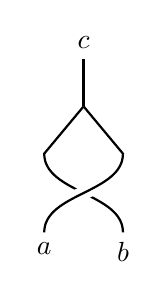
\begin{tikzpicture}[thick, baseline=(current bounding box.center)]
  \draw (1,0) node[below] {$b$} .. controls (1,0.5) and (0,0.5) .. (0,1) -- (0.5,1.6);
  \draw[white, line width=5pt] (0,0) .. controls (0,0.5) and (1,0.5) .. (1,1);
  \draw (0,0) node[below] {$a$} .. controls (0,0.5) and (1,0.5) .. (1,1) -- (0.5,1.6);
  \draw (0.5,1.6) -- (0.5,2.2) node[above] {$c$};
\end{tikzpicture}
\;=\; R^{ab}_c
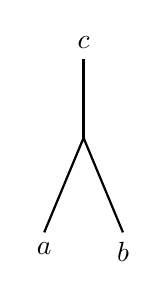
\begin{tikzpicture}[thick, baseline=(current bounding box.center)]
  \draw (0,0) node[below] {$a$} -- (0.5,1.2) -- (1,0) node[below] {$b$};
  \draw (0.5,1.2) -- (0.5,2.2) node[above] {$c$};
\end{tikzpicture}$
